\documentclass[12pt]{article}
\usepackage{graphicx}
\usepackage{caption}
\usepackage{amsmath}
\usepackage{geometry}
\usepackage{float}
\usepackage{booktabs}
\usepackage{longtable}
\usepackage{setspace} % for spacing control
\usepackage{indentfirst}
\usepackage{titlesec}
\setstretch{1.0}       % single line spacing (default)
\setlength{\parskip}{0pt}   % no space between paragraphs
\setlength{\parindent}{0em} % set indentation amount

\geometry{margin=1in}
\setlength{\parskip}{0em}
\setlength{\parindent}{0pt}

\title{Assignment 1 \\ \large Computational Plasticity (SoSe25)}
\author{Bagus Alifah Hasyim \\ 108023246468 \\ Last Three Digits: 468}
\date{}

\begin{document}
\maketitle

\section*{Given Data}
\hspace*{2em}In this section we need to define every data that is given in the assignment, such as the material properties, geometry, 
and other relevant parameters that are needed for the analysis. Therefore, following data shall we define using the author's "immatrikulation nummer":

\begin{itemize}
    \item $E_a = 200 + (10 \times 4) = 240 \;\text{GPa}$  
    \item $\sigma_a = 300 + (10 \times 6) = 360 \;\text{MPa}$
    \item $\sigma_{yb} = 200 + (10 \times 8) = 280 \;\text{MPa}$
\end{itemize}

\section{Introduction}
\hspace*{2em}In this assignment, we will analyze the mechanical response of a baseline plate
and a plate with a circular inclusion under uniaxial loading. 
The analysis will include comparison of obtaining stress-strain curves between the force-displacement and
direct stress-strain curves, differentiating plane stress and plane strain conditions, comparing 
local stress field distribution based on different constitutive models, and evaluating stress at specific points based on mesh sizes.

\hspace*{2em}For the following sections we will systematically address each question in the assignment, 
providing detailed explanations, derivations, and relevant figures or tables to 
support the analysis. 
All calculations and results are based on the provided data and the author's unique 
identification number. Numerical analysis will be performed using Abaqus CAE with an appropriate
boundary condition and settings. 

\section{Set up of the Model}
\hspace*{2em}For the model setup, we will use Abaqus CAE to create a 2D planar-deformable shell model of the plate with the specified geometry, boundary condition, material properties, and mesh.  
\subsection{Geometry and Boundary Conditions}
%add axis in the figure, for direction 1, 2, and 3
\begin{enumerate}
     \item \textbf{Baseline Plate:} A rectangular plate with length $L = 40 \;\text{mm}$, width $W = 10 \;\text{mm}$, and thickness $t = 1 \;\text{mm}$.
        \begin{figure}[H]
        \centering
            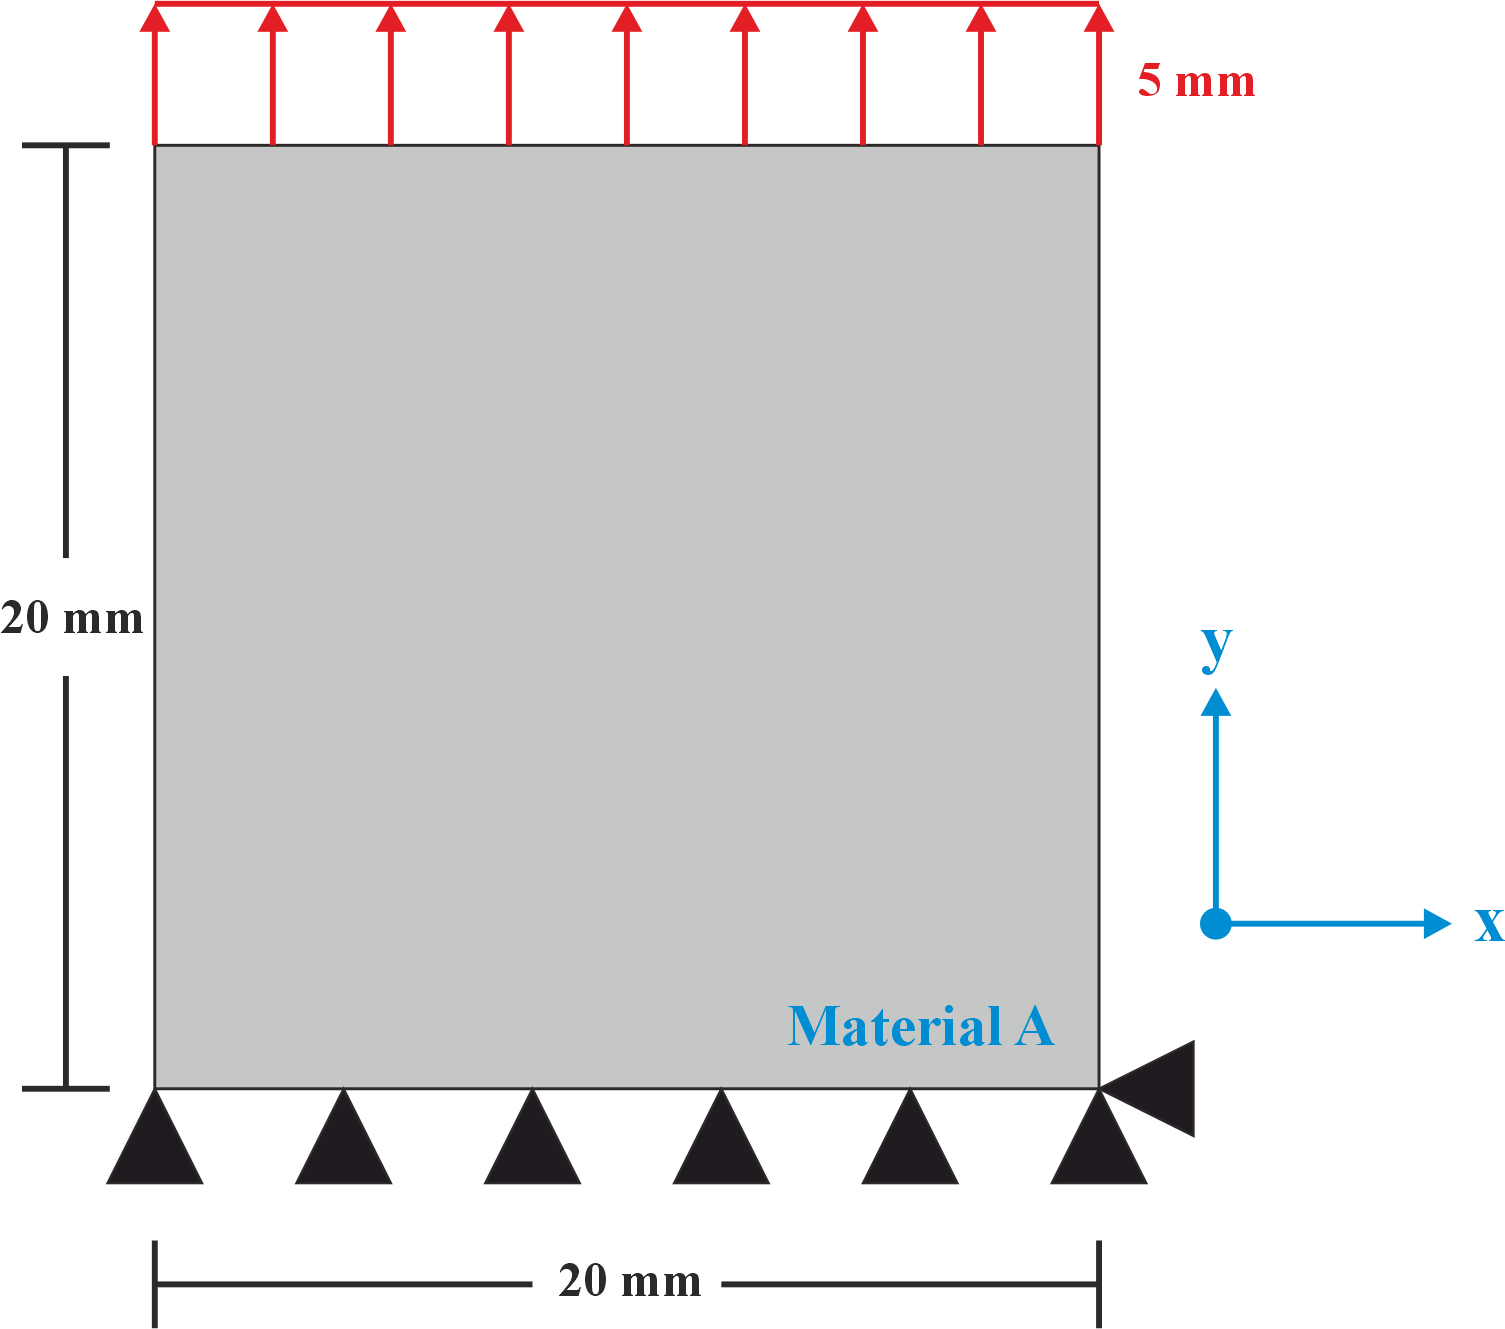
\includegraphics[width=0.5\textwidth]{images/TaskQ1.png}
        \caption{Baseline plate geometry with defined material A. Two boundary conditions are applied, which are the 
        fixed support restriction in y direction on the bottom line of the plate, fixed support point on the bottom right point,
        and constant distribution of displacement in y direction on the top line of the plate, which has value of 5 mm.}
        \label{fig:geometryQ1}
\end{figure}

    \item \textbf{Plate with Circular Inclusion:} Same as the baseline plate, but with a circular inclusion of radius $r=4$ mm located at the center or specified position.
\begin{figure}[H]
        \centering
            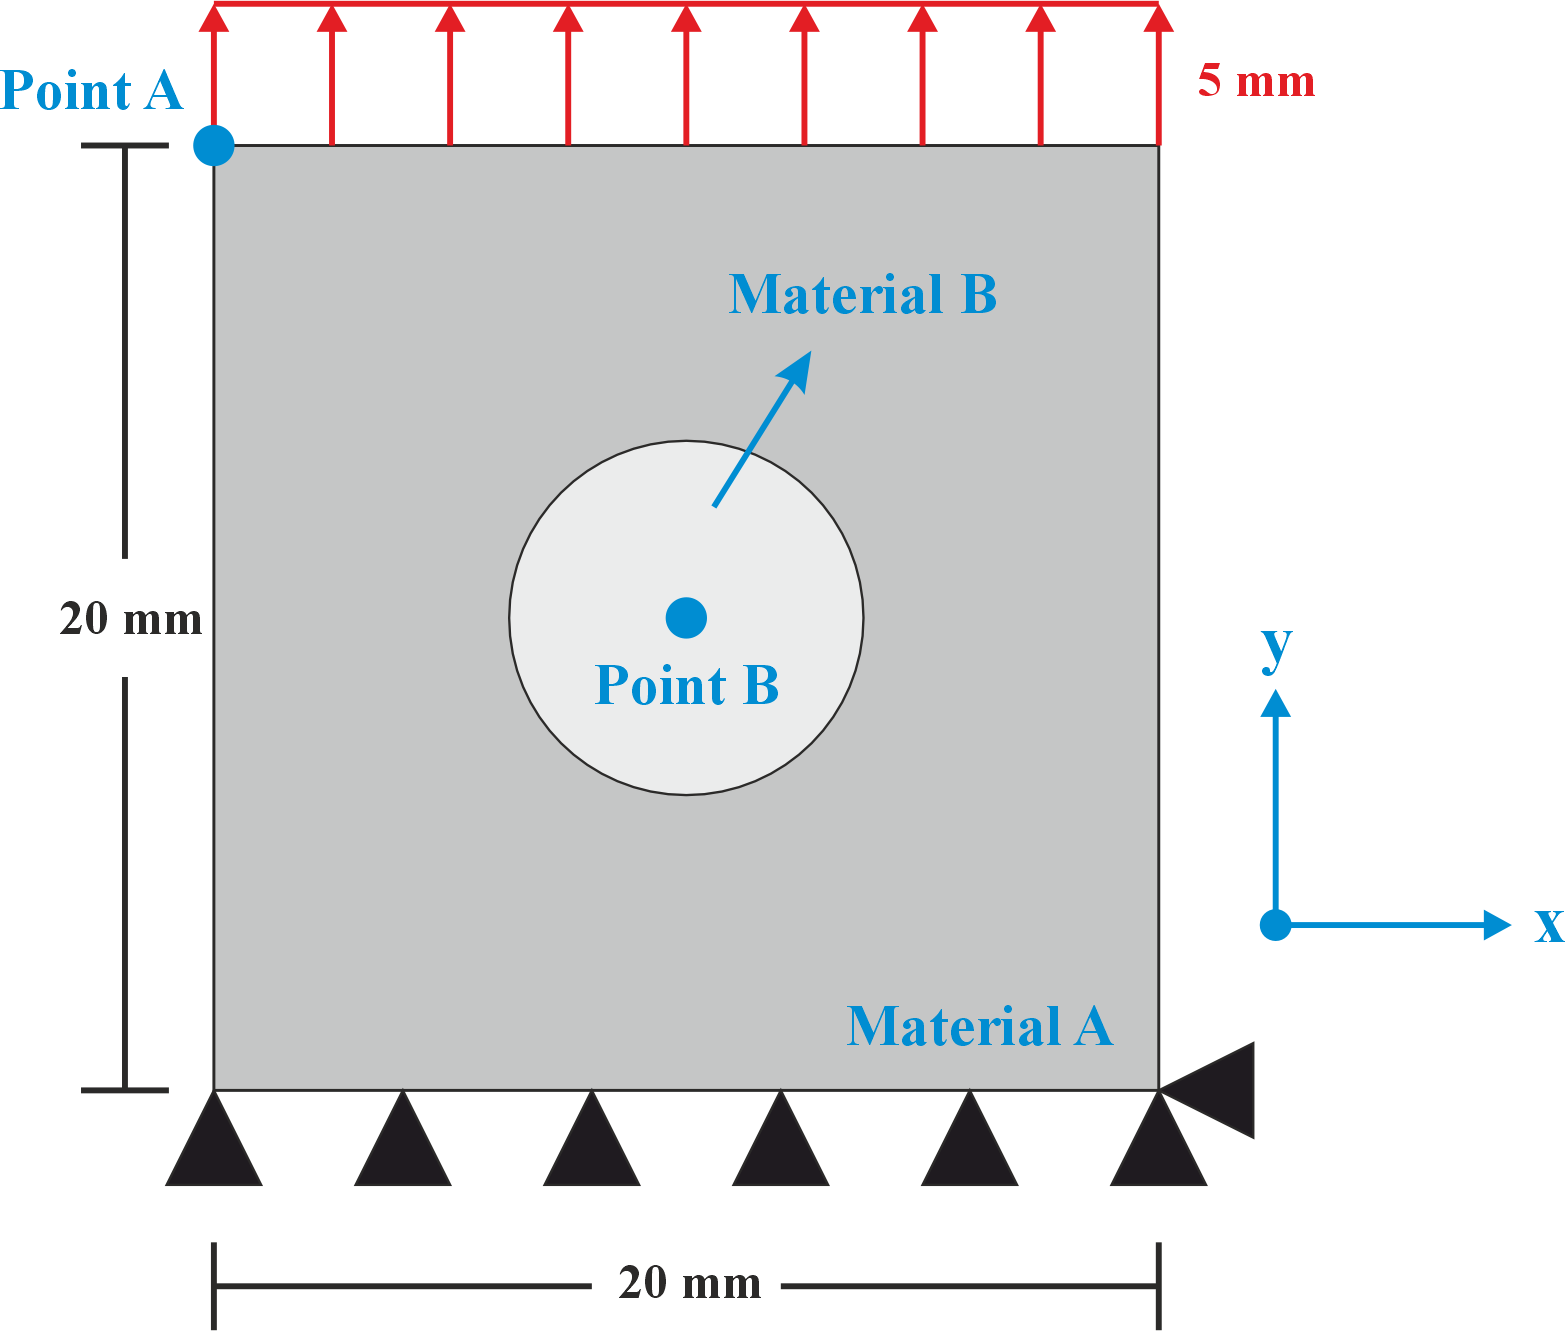
\includegraphics[width=0.52\textwidth]{images/TaskQ2.png}
        \caption{Plate with circular inclusion and defined material B. Boundary conditions are the same as in Task 1 shown in Figure~\ref{fig:geometryQ1}.}
        \label{fig:geometryQ2}
\end{figure}
\end{enumerate}
\subsection{Material Properties}
\hspace*{2em}Material properties for the analysis are provided from the task definition, which there are some
material parameters that need to be manually calculated based on the author's Immatrikulation Nummer in at very 
first section. 
For task 1, material A (see Table~\ref{tab:materialA-properties}) will be used and defined as an elastic-plastic material with properties based on the Young's modulus $E$, Poisson's ratio $\nu$, and yield stress $\sigma_{ya}$,
and ultimate tensile strength $\sigma_{f}$, and the strain at fracture $\epsilon_{f}^{f}$ in isotropic condition.   
For task 2 with additional inclusion material B in the center, it is defined as an elastic-plastic material with anisotropic properties, 
which it defines the properties differently in three orthogonal directions. Especially for the plastic properties in table~\ref{tab:materialB-plasticproperties},
it used Hill's yield criterion, which is defined by the Hill's coefficients $R_{ij}$, where $i,j = 1,2,3$ for the three orthogonal directions. 


\begin{table}[H]
    \centering
    \caption{Elastic and plastic properties of material A.}
    \label{tab:materialA-properties}
    \begin{tabular}{lllll}
        \toprule
        E (GPa) & $\nu$ & $\sigma_{ya}$ (MPa) & $\sigma_{f}$ (MPa) & $\epsilon_{f}^{f}$ \\
        \midrule
        240 & 0.3 & 360 & 550 & 0.4 \\
        \bottomrule
    \end{tabular}
\end{table}

\begin{table}[H]
    \centering
    \caption{Elastic properties of material B.}
    \label{tab:materialB-elasticproperties}
    \begin{tabular}{lllllllll}
        \toprule
            \centering $E_1$ (GPa) & $E_2$ (GPa) & $E_3$ (GPa) & $\nu_{12}$ & $\nu_{13}$ & $\nu_{23}$ & $G_{12}$ (MPa) & 
            $G_{13}$ (MPa) & $G_{23}$ (MPa) \\
            \midrule
            \centering 210 & 220 & 230 & 0.3 & 0.31 & 0.32 & 80 & 84 & 87 \\
            \bottomrule
    \end{tabular}
\end{table}

\begin{table}[H]
    \centering
    \caption{Plastic properties of material B.}
    \label{tab:materialB-plasticproperties}
    \begin{tabular}{lllllllll}
        \toprule
            \centering $R_{11}$ & $R_{22}$ & $R_{33}$ & $R_{12}$ & $R_{13}$ & $R_{23}$ & $\sigma_{yb}$ & 
            $\sigma_{f}$ (MPa) & $\epsilon_{p}^{f}$  \\
            \midrule
            \centering 1 & 1.2 & 1.25 & 0.8 & 0.85 & 0.95 & 280 & 450 & 0.5 \\
            \bottomrule
    \end{tabular}
\end{table}
\subsection{Meshing}
\hspace{2em}The models for this tasked are differentiate into two different 
meshes types, which first one is the homogeneous baseline plate 
with a uniform mesh size distribution, and the 
second one is the plate with circular inclusion,
which it has a customized mesh distribution in order to 
take account creating symmetrical meshes distribution 
across the geometry variant. Creating meshes for geometry with inclusion
should be taking care of some aspects, for instance, defining the distribution 
pattern of the mesh size, which the program mesh algorithm from Abaqus
CAE can automatically generate a symmetrical mesh distribution. Hence, 
defining geometry partition is having an important role in order to achieve
a good mesh distribution. The following figures show the meshing
for both models. Noted that in this assignment, we will not use the
reduced integration element, which in the end the logaritihmic strain
will be shown instead of the regular strain. 
\begin{figure}[H]
    \centering
    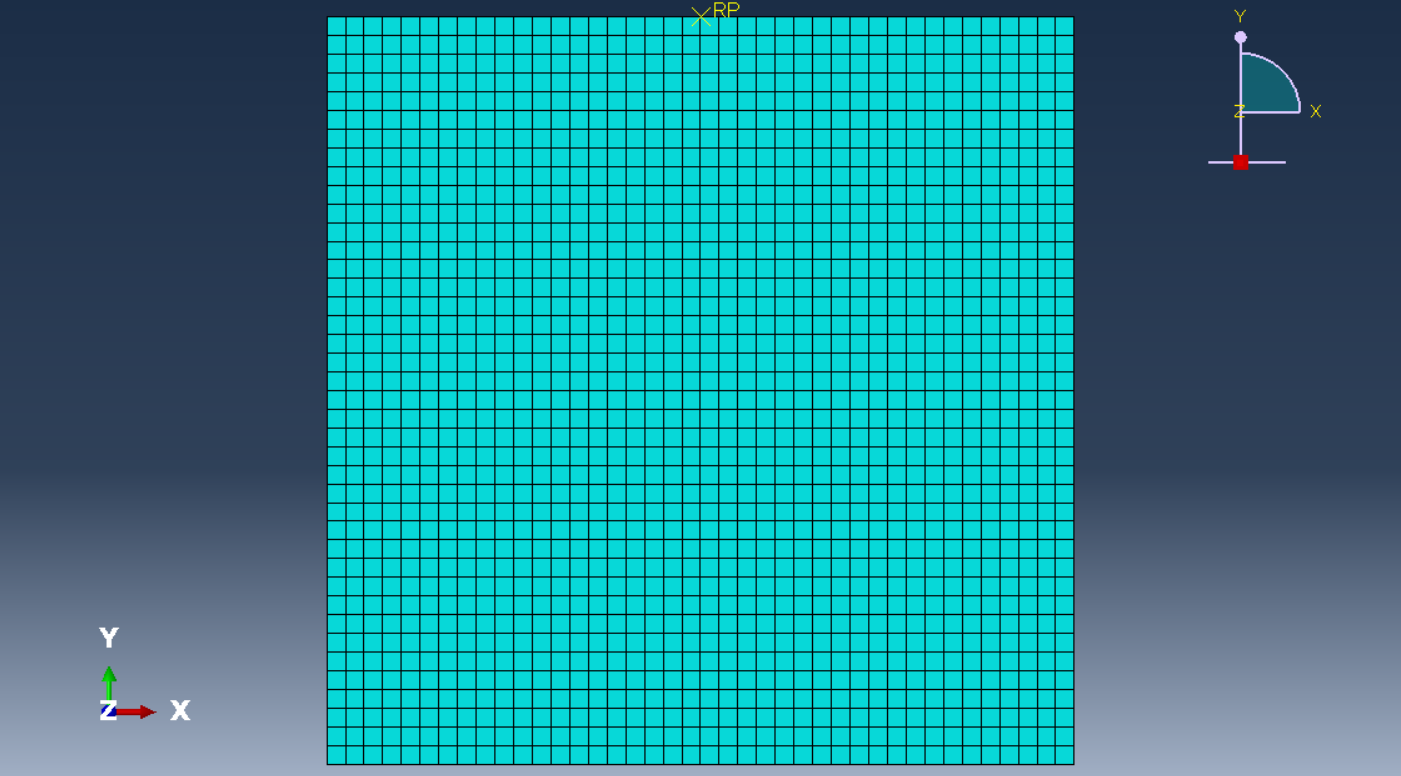
\includegraphics[width=1\textwidth]{images/MeshQ1.png}
    \caption{Mesh for the baseline plate with uniform mesh size distribution, 
    with total of 1600 elements. The mesh size is defined as 0.25 mm
    gap size with set up for both plane stress and plane strain
    conditions.}
    \label{fig:MeshQ1}
\end{figure}

\begin{figure}[H]
    \centering
    \begin{minipage}{0.48\textwidth}
        \centering
        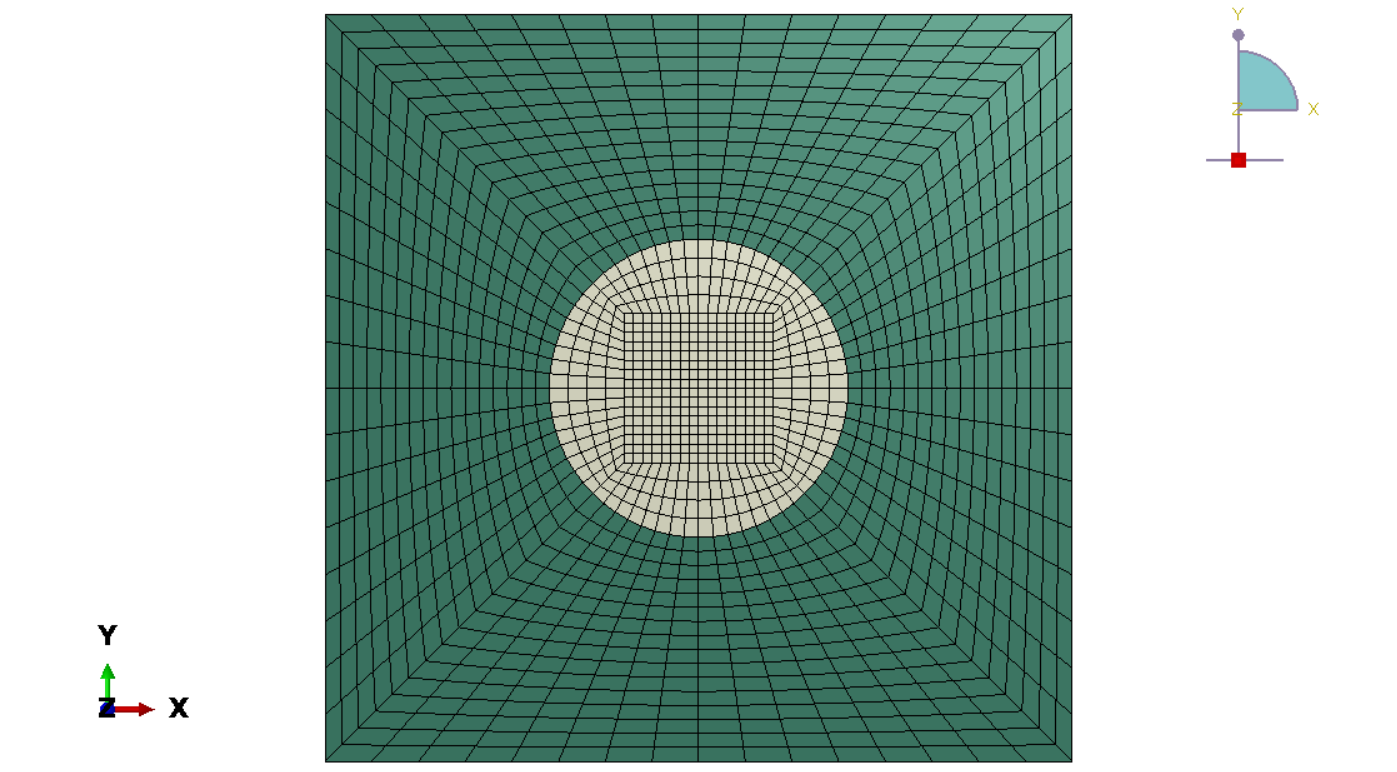
\includegraphics[width=\textwidth]{images/MeshQ2.1.png}
        \caption{Mesh for the plate with circular inclusion for the coarse variation
        with 1536 elements.}
        \label{fig:MeshQ2.1}
    \end{minipage}\hfill
    \begin{minipage}{0.48\textwidth}
        \centering
        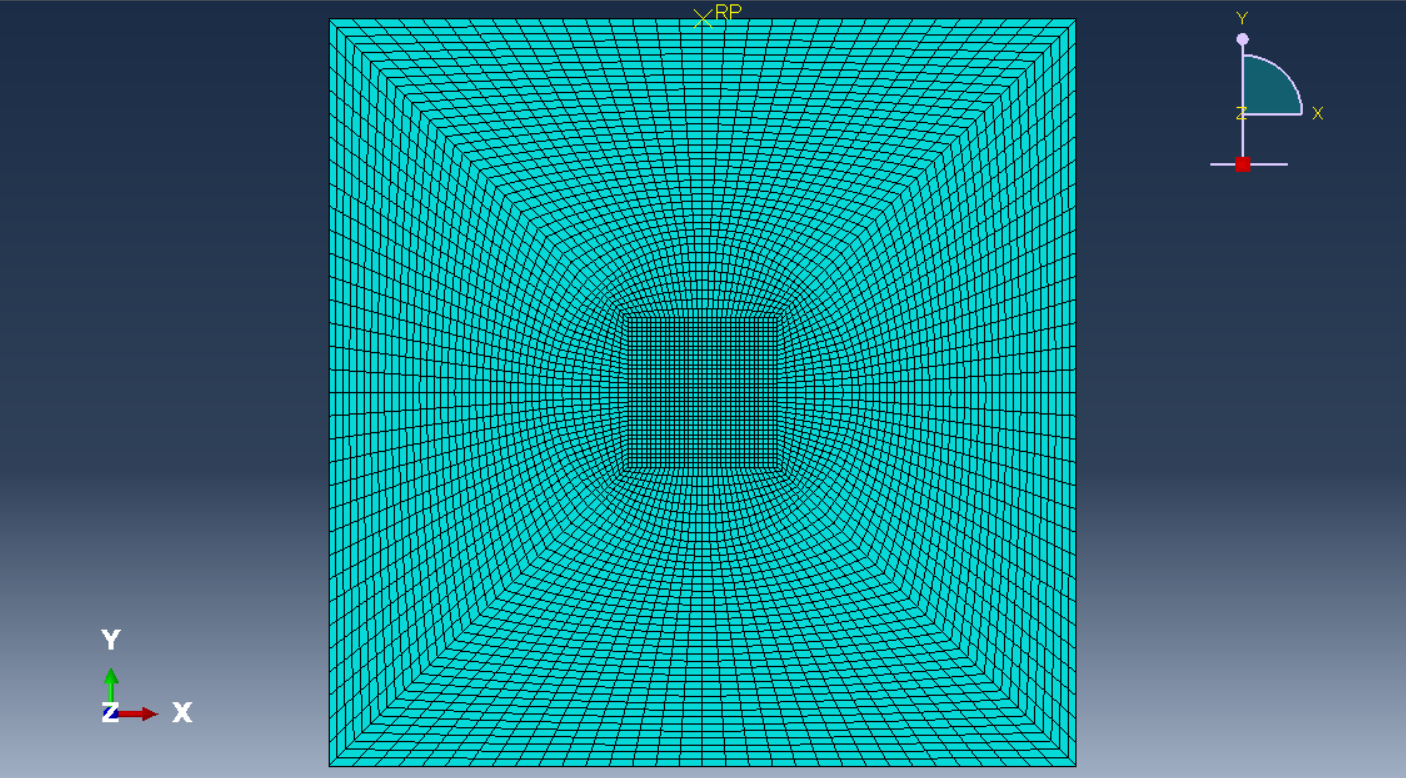
\includegraphics[width=\textwidth]{images/MeshQ2.2.png}
        \caption{Mesh for the plate with circular inclusion for fine mesh variation
        with 6144 elements.}
        \label{fig:MeshQ2.2}
    \end{minipage}
\end{figure}
\section*{Results and Discussion}

\subsection*{Q1: Mechanical Response Analysis for Baseline Plate}
\begin{figure}[H]
    \centering
    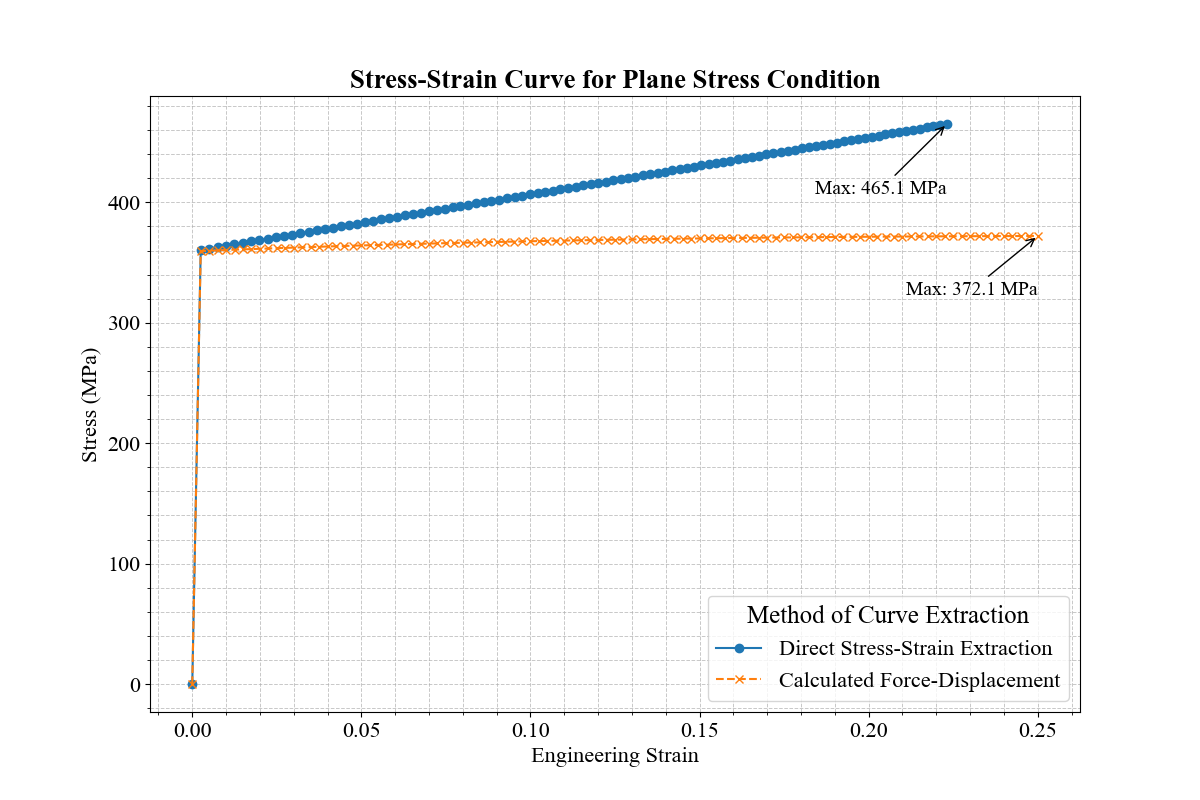
\includegraphics[width=1\textwidth]{visualize_tensileGraph/res/comparison_direct_calculated.png}
    \caption{Comparison of
    the stress-strain curves obtained from the force-displacement method and the direct stress-strain calculation
    for plane stress condition. The direct stress-strain curve method is obtained 
    by extracting the stress $\sigma_{22}$ and strain $\varepsilon_{22}$ directly from the 
    history output, which are the whole nodes along the top edges of the baseplate. While the caculated
    Force-Displacement is obtained by extracting the force 
    $F_{22}$ and displacement $U_{22}$ from the history output, which are the whole nodes along the top edges of the baseplate.
    Then the stress is obtained by dividing the force with the surface area
    normal to the loading direction, which is A = 20 $mm^2$. While the strain is calculated by obtaining the displacement,
    which then it will be divided by the baseplate original length, which is L = 20 $mm$, with respect to the loading
    direction.} 
    \label{fig:ComparisonDirectCalculated}  
\end{figure}
    \hspace{2em}Based on Figure~\ref{fig:ComparisonDirectCalculated}, both stress-strain curves obtained from the two 
    methods show different behavior. In the plastic region, the direct method produces a significant slope 
    in the plastic flow region, while the calculated method shows a constant slope, 
    indicating the material behaves as perfectly plastic without hardening. 
    This difference occurs because, in the first method, the solver calculates the true stress-strain 
    by accounting for changes in geometric properties such as the cross-sectional area. In the plastic 
    region, the geometry undergoes necking, which decreases the cross-sectional area and leads to higher 
    stress values. This method is often called the true stress-strain diagram, as it uses the logarithmic 
    strain and accounts for the reduction in cross-sectional area.

\hspace{2em}In the second method, the stress obtained by calculating the total force produced in the top nodal line of the baseplate divided by a constant area value, which here
the stresses are most likely does not increase in the plastic region, since it use the original cross-sectional area as the dominator. This method also applied to calculate the strain, which only
divide the displacement with the original length of the baseplate. This method is often use to create the engineering stress-strain curve. In the experimental tensile test, 
this method oftenly used to obtain the stress-strain curve, since the obtained test data is only force and displacement of the extensiometer. 

\begin{figure}[H]
    \centering
    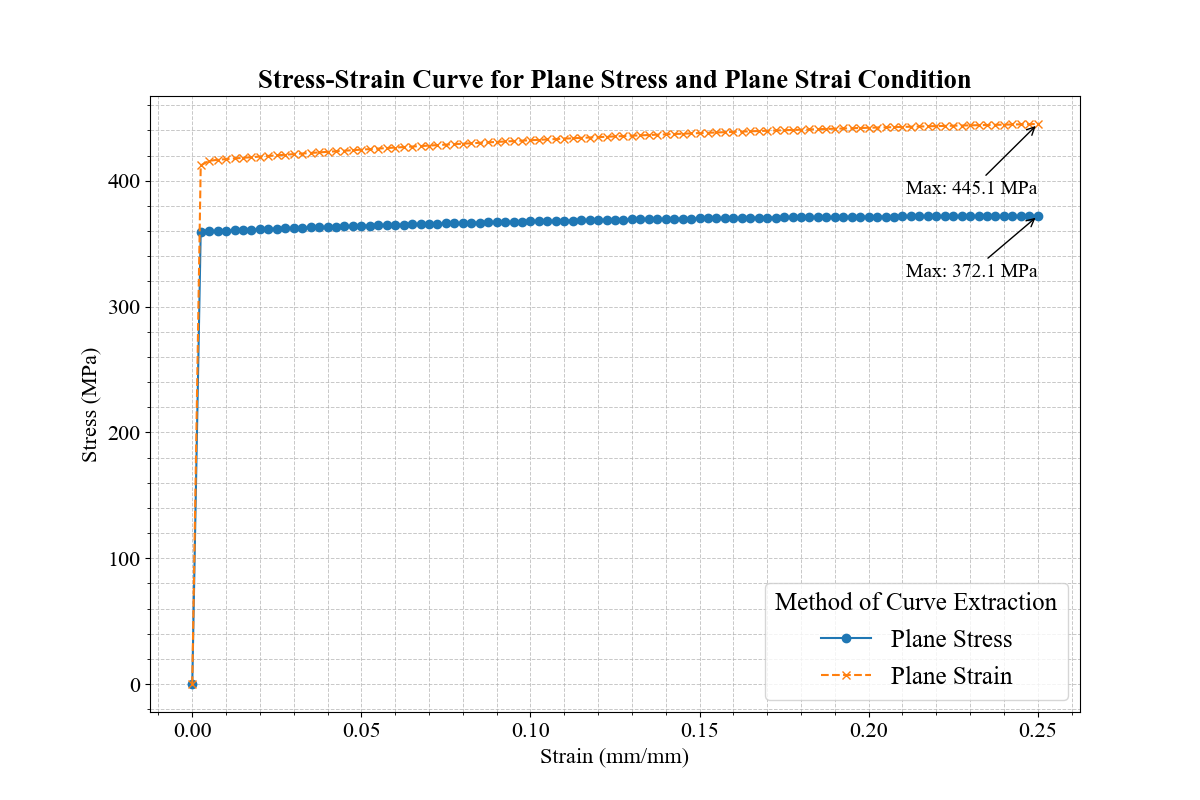
\includegraphics[width=1\textwidth]{visualize_tensileGraph/res/comparison_planeStress_planeStrain.png}
    \caption{Comparison of plane stress and plane strain conditions
    for the baseline plate with material A. The setting for plane stress and strain are distinguised by changing the type of meshing in
    Abaqus based on the condition.} 
    \label{fig:ComparisonDirectCalculated}  
\end{figure}
\hspace{2em}Based on Figure~\ref{fig:ComparisonDirectCalculated}, the stress-strain curves for both plane stress and plane strain conditions show similar behavior, with the plane strain condition exhibiting a slightly higher yield stress.
This is expected, as the plane strain condition restricts deformation in the thickness direction, 
leading to higher stress values. This stress produced since the strain restriction in the thickness
will cause additional stress component that will increase the stress in the loading direction. Therefore, choosing the 
plane stress condition is more appropriate for thin-plates analysis since it neglects stress generated 
in the thickness direction. 

\subsection*{Q2: Mechanical Response Analysis for Plate with Circular Inclusion}

In this section, we analyze the mechanical response of the plate with a circular inclusion and compare it to the homogeneous baseline plate.

\begin{figure}[H]
    \centering
    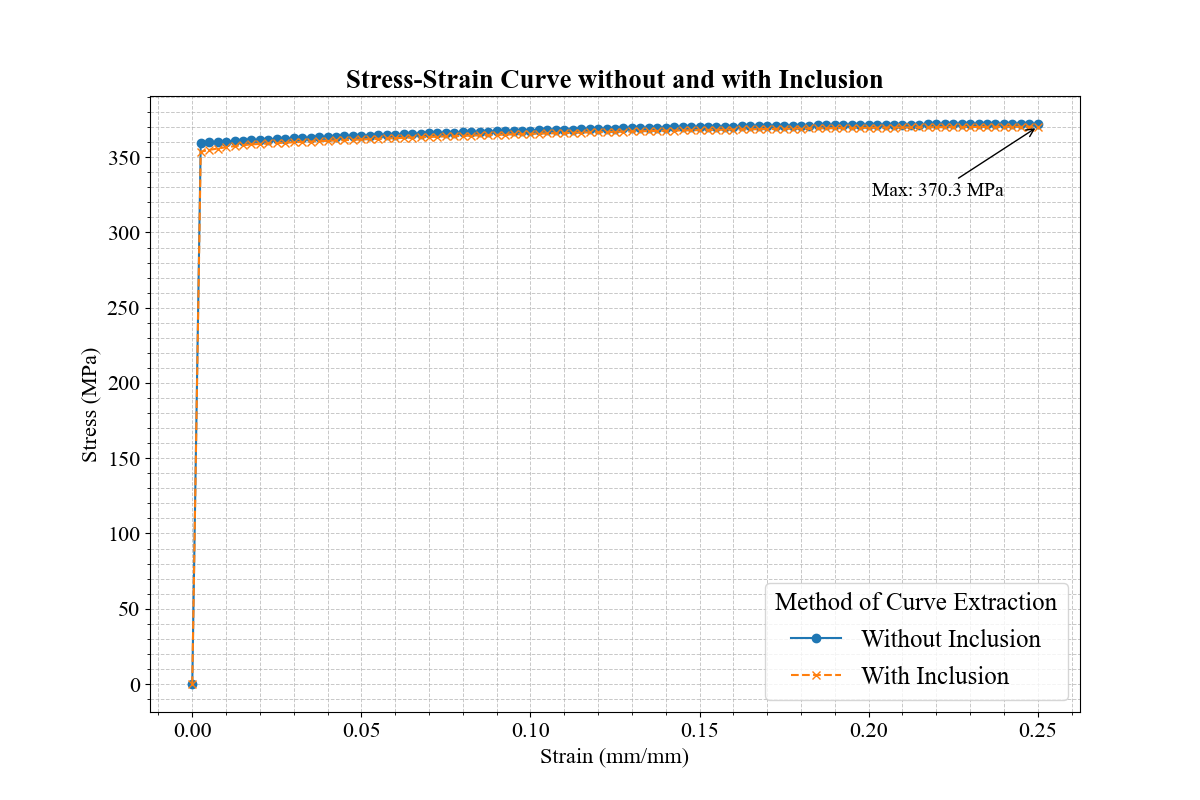
\includegraphics[width=1\textwidth]{visualize_tensileGraph/res/comparison_inclusion_non.png}
    \caption{Comparison of the stress-strain curves for the homogenous baseplate and plate with circular
    inclusion.}
    \label{fig:ComparisonInclusion}
\end{figure}

\hspace{2em}From the response of the stress-strain curves for each plate, we can see that the plate with inclusion
has a lower yield stress compared to the homogeneous plate. This cause by the material B inclusion's yield stress having
lower value compare to the material A, which is 280 MPa. This will reduce the overall yield stress of the whole plate, 
which will make the material softer compared to the homogeneous plate only using material A. 

\hspace{2em}This reduction of overall stress is also applied in the maximum stress for the plate with inclusion, which also decrease in terms of value.
The reason for this is because material B has a lower ultimate tensile stress compare to material A, which is 450 MPa and 550 MPa, respectively. Hence, the
stress reduction is not in a huge difference, since the inclusion does not dominantly affect the overall tensile stress.

\hspace{2em}In addition, the plate with inclusion shows simmilar behavior in the elastic
region despite there is difference in the value of young's modulus between material A and B. Here, material A's young's modulus is dominating
the role so that the overall elastic response for the plate with inclusion does not decrease. 

\subsection*{Q3: Local Stress Field Distribution and Analysis}
Hence, we will analyze the stress distribution for baseplates with inclusion. 
\begin{figure}[H]
    \centering
    \begin{minipage}{0.48\textwidth}
        \centering
        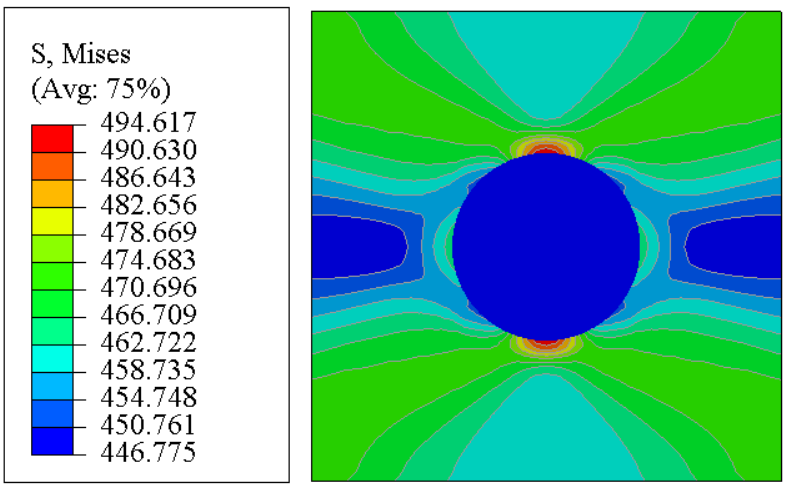
\includegraphics[width=\textwidth]{images/MISES.png}
        \caption*{(a) $\sigma_{vM}$}
    \end{minipage}
    \hfill
    \begin{minipage}{0.48\textwidth}
        \centering
        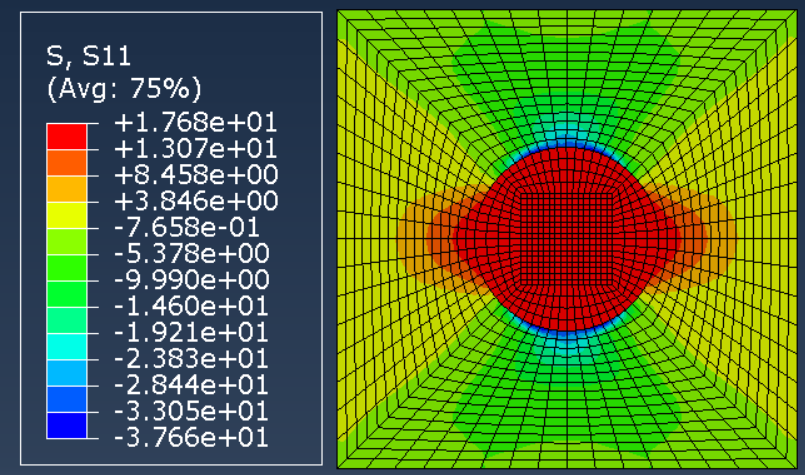
\includegraphics[width=\textwidth]{images/S11.png}
        \caption*{(b) $S_{11}$}
    \end{minipage}
    \vspace{1em}
    \begin{minipage}{0.48\textwidth}
        \centering
        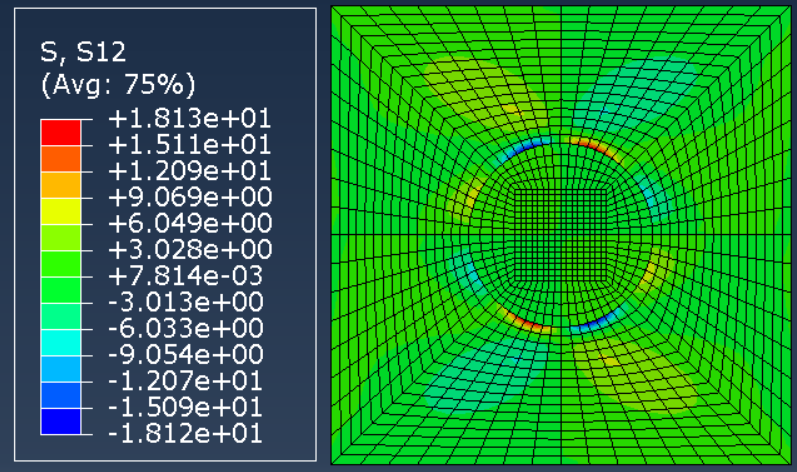
\includegraphics[width=\textwidth]{images/S12.png}
        \caption*{(c) $S_{12}$}
    \end{minipage}
    \hfill
    \begin{minipage}{0.48\textwidth}
        \centering
        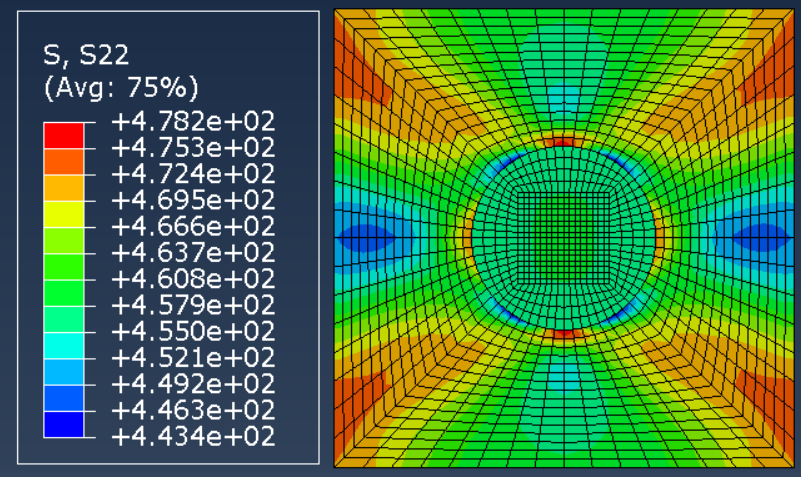
\includegraphics[width=\textwidth]{images/S22.png}
        \caption*{(d) $S_{22}$}
    \end{minipage}
    \caption{Contour plots of (a) von Mises stress, (b) $S_{11}$, (c) $S_{12}$, and (d) $S_{22}$ for the plate with circular inclusion.}
    \label{fig:stressFields}
\end{figure}

\hspace{2em}From the stress distribution contour plots in Figure~\ref{fig:stressFields},
we can see some several characteristics of the stress behavior in the plate with circular inclusion.
\begin{itemize}
    \item In the von Misses stress in part (a), it shows a discontinuity stress distribution between the inclusion
    and the outer of the non-inclusion part. This is because both material A as in the non-inclusion and material B
    having the different material properties, which material B tends to be softer compare to material A.
    Therefore, it can easily deform and hence will produce a lower stress.
    \item As in the $S_{11}$ distribution, the stress tends to have negative value for the non-inclusion area.
    This is because as the plate deform, the specimen will getting squized to the right side, parallel to x axis.
    Hence, it will produce a reaction force opposite to the movement, and will produce a negative value of stress, 
    which indicates that the material is getting compressed in the x direction.
    \item In the $S_{12}$ plot, the shear stress value tends to be small in the whole part of the plate. However, there
    are some shear stress generated in the boundary between the inclusion and the homogeneous part of the
    plate, which here causes by the friction between two different material.
    \item For the stress plot in the y direction, which is $S_{22}$, the highest stress mostly generated in the 4 edges
    of material A and in between material A and inclusion material B.  
\end{itemize}

\subsection*{Q4: Comparison Analysis at Point A}
To calculate the von Misses equivalent stress and equivalent plastic strain at point A analytically, 
we can use following equations:
\begin{equation}
    \sigma_{eq, hill} = \sqrt{
        F(\sigma_{22}-\sigma_{33})^2 + 
        G(\sigma_{33}-\sigma_{11})^2 + 
        H(\sigma_{11}-\sigma_{22})^2 + 
        2L\sigma_{23}^2 + 
        2M\sigma_{31}^2 + 
        2N\sigma_{12}^2
    }
    \label{eq:hill_yield}
\end{equation}

\begin{equation}
    \varepsilon_{eq} = \sqrt{\frac{F\varepsilon_{pl,11}^2 + G\varepsilon_{pl,22}^2 + H\varepsilon_{pl,33}^2}{FG+FH+GH} + \frac{2\varepsilon_{pl,12}^2}{N}}
    \label{eq:equivalent_plastic_strain}
\end{equation}

where $\varepsilon_{pl,33}=-(\varepsilon_{pl,11}+\varepsilon_{pl,22})$. Hence all of the constant in the equations
are described using $R_{ij}$, where these variable describe the ratio of plasticity between the preceeding directions and the based
yield stress:

\begin{align*}
F &= \frac{1}{2} \left[ \frac{1}{(R_{22})^2} + \frac{1}{(R_{33})^2} - \frac{1}{(R_{11})^2} \right] \\
G &= \frac{1}{2} \left[ \frac{1}{(R_{33})^2} + \frac{1}{(R_{11})^2} - \frac{1}{(R_{22})^2} \right] \\
H &= \frac{1}{2} \left[ \frac{1}{(R_{11})^2} + \frac{1}{(R_{22})^2} - \frac{1}{(R_{33})^2} \right] \\
L &= \frac{3}{2(R_{23})^2} \\
M &= \frac{3}{2(R_{31})^2} \\
N &= \frac{3}{2(R_{12})^2}
\end{align*}

At point A, since it use material A and it is an isotropic material, 
therefore we can assume all of the $R_{ij}$ are equal to 1. Therefore, the hill's
equivalent stress and strain can be simplified as follows:
\begin{equation}
    \sigma_{eq, hill} = \sqrt{\frac{1}{2}((\sigma_{22}-\sigma_{33})^2 + (\sigma_{33}-\sigma_{11})^2 + (\sigma_{11}-\sigma_{22})^2 + 6\sigma_{23}^2 + 6\sigma_{31}^2 + 6\sigma_{12}^2)}
\end{equation}
\begin{equation}
    \varepsilon_{eq} = \sqrt{\frac{2(\varepsilon_{pl,11}^2 + \varepsilon_{pl,22}^2 + (\varepsilon_{pl,11}+\varepsilon_{pl,22})^2)}{3} + \frac{4\varepsilon_{pl,12}^2}{3}}
\end{equation}

At point A, the value of the stress and strain can be extracted directly from Abaqus. Following is the tabulized result for each 
variable that are needed for the calculation.
\begin{table}[H]
    \centering
    \caption{Extracted stress and strain components at point A from Abaqus.}
    \label{tab:pointA-results}
    \begin{tabular}{llllll}
        \toprule
        $\sigma_{11}$ (MPa) & $\sigma_{22}$ (MPa) & $\sigma_{12}$ (MPa) & $\varepsilon_{pl,11}$ & $\varepsilon_{pl,22}$ & $\varepsilon_{pl,12}$\\
        \midrule
        -2.61 & 472.16 & 1.24 & -0.1196 & 0.2388 & -0.0014\\
        \bottomrule
    \end{tabular}
\end{table}

Then we can use these data to calculate the equivalent von Mises stress and plastic strain. 

\begin{equation}
    \sigma_{eq, hill}^A = \sqrt{\frac{1}{2}((\sigma_{22}-0)^2 + (0-\sigma_{11})^2 + (\sigma_{11}-\sigma_{22})^2 + 6\sigma_{12}^2)} 
\end{equation}

\begin{equation}
    \sigma_{eq, hill}^A = \sqrt{\frac{1}{2}((472.16-0)^2 + (0-(-2.61))^2 + ((-2.61)-472.16)^2 + 6(1.24)^2)}
\end{equation}
\begin{equation}
    \sigma_{eq, hill}^A = 473.592 \; \text{MPa}
\end{equation}

\begin{equation}
    \varepsilon_{eq}^A = \sqrt{\frac{2((-0.1196)^2 + (0.2388)^2 + ((-0.1196)+(0.2388))^2)}{3} + \frac{4(-0.0014)^2}{3}}
\end{equation}
\begin{equation}
    \varepsilon_{eq}^A = 0.2388
\end{equation}

\hspace{2em}Therefore, we obtain the Hill's equivalent stress 473.592 MPa and the equivalent strain of
0.2388 at point A. From the simulation results, the equivalent von Mises stress at point A
is $\sigma_{A} = 473.478 \; \text{MPa}$, while the equivalent plastic strain (PEEQ) is 
$\varepsilon_{A} = 0.2388$ from probing directly the node at point A in Abaqus. Hence, we can see
simmilar result for both stress and strain value, but there lies a different value between
the calculated stress and the obtained stress, which here cause by the rounding-off error.

    \begin{figure}[H]
    \centering
    \begin{minipage}{0.48\textwidth}
        \centering
        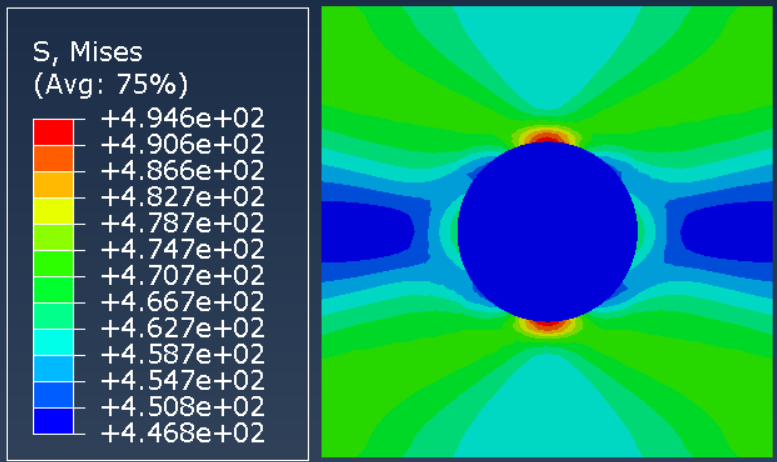
\includegraphics[width=\textwidth]{images/MISES_Coarse.png}
        \caption*{(a) $\sigma_{vM}$ for coarse mesh}
    \end{minipage}
    \hfill
    \begin{minipage}{0.48\textwidth}
        \centering
        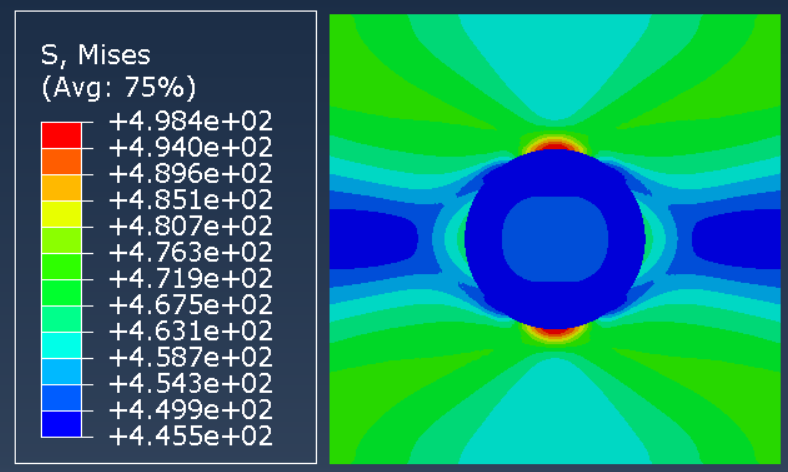
\includegraphics[width=\textwidth]{images/MISES_Fine.png}
        \caption*{(b) $\sigma_{vM}$ for fine mesh}
    \end{minipage}
    \vspace{1em}
    \begin{minipage}{0.48\textwidth}
        \centering
        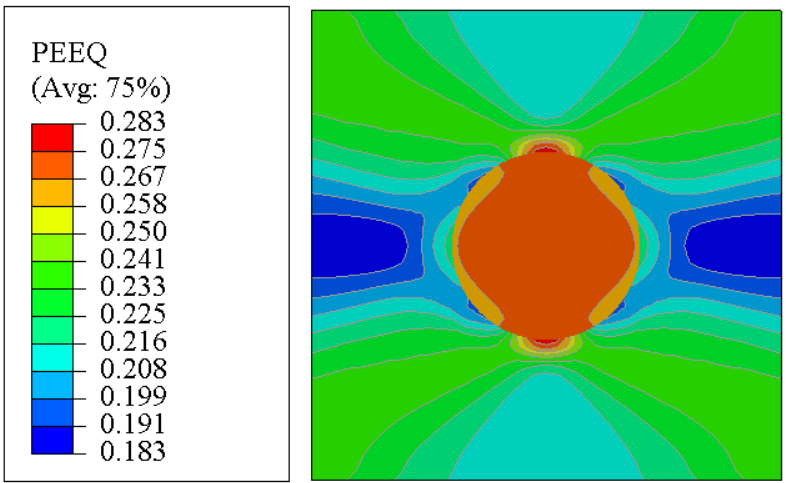
\includegraphics[width=\textwidth]{images/PEEQ_Coarse.png}
        \caption*{(c) $\varepsilon_{vM}$ for coarse mesh}
    \end{minipage}
    \hfill
    \begin{minipage}{0.48\textwidth}
        \centering
        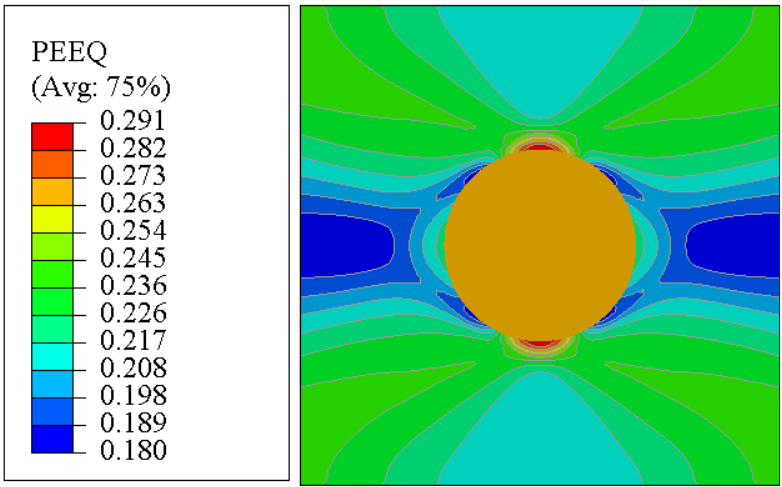
\includegraphics[width=\textwidth]{images/PEEQ_Fine.png}
        \caption*{(d) $\varepsilon_{vM}$ for fine mesh}
    \end{minipage}
    \caption{Comparison of von misses stress and equivalent plastic strain distribution 
    for coarse (a, c) and fine (b, d) mesh 
    sizes for 1536 and 6144 nodes, respectively.}
    \label{fig:stressFields}
\end{figure}
\hspace{2em}As we employed a mesh refining process, both of the stresses and strains for both the maximum value
are increase. But if we compare the stress at point A, using the finer mesh the value will decrease to $\sigma_{A}^{fine}=473.28 \; \text{MPa}$,
while the PEEQ strain also decreasing but in a small amount to $\varepsilon_{A}^{fine} = 0.2385$.
Hence refining the mesh can change the resulting value. In this case, it only change in a small amount, where it
can be concluded as a small mesh sensitivity analysis, the mesh does not influence the
generating results of both stress and strain values. 

\subsection*{Q5: Comparison Analysis at Point B}
Using equation~\ref{eq:hill_yield} and~\ref{eq:equivalent_plastic_strain}, we can calculate the Hill's equivalent stress and 
equivalent plastic strain at point B analytically. First, we need to extract the stress and strain
components from Abaqus using the same method as in the previous question 4. Following are the extracted value
at point B:

\begin{table}[H]
    \centering
    \caption{Extracted stress and strain components at point B from Abaqus.}
    \label{tab:pointA-results}
    \begin{tabular}{llllll}
        \toprule
        $\sigma_{11}$ (MPa) & $\sigma_{22}$ (MPa) & $\sigma_{12}$ (MPa) & $\varepsilon_{pl,11}$ & $\varepsilon_{pl,22}$ & $\varepsilon_{pl,12}$\\
        \midrule
        15.74 & 458.18 & 0 & -0.1629 & 0.2555 & 0\\
        \bottomrule
    \end{tabular}
\end{table}

For F, G, and H, we can use the values from the material B properties
\begin{align*}
F &= \frac{1}{2} \left[ \frac{1}{(R_{22})^2} + \frac{1}{(R_{33})^2} - \frac{1}{(R_{11})^2} \right] = \frac{1}{2} \left[ \frac{1}{(1.2)^2} + \frac{1}{(1.25)^2} - \frac{1}{(1)^2} \right] = 0.1672\\
G &= \frac{1}{2} \left[ \frac{1}{(R_{33})^2} + \frac{1}{(R_{11})^2} - \frac{1}{(R_{22})^2} \right] = \frac{1}{2} \left[ \frac{1}{(1.25)^2} + \frac{1}{(1)^2} - \frac{1}{(1.2)^2} \right] = 0.4728\\
H &= \frac{1}{2} \left[ \frac{1}{(R_{11})^2} + \frac{1}{(R_{22})^2} - \frac{1}{(R_{33})^2} \right] = \frac{1}{2} \left[ \frac{1}{(1)^2} + \frac{1}{(1.2)^2} - \frac{1}{(1.25)^2} \right] = 0.5277
\end{align*}    

Therefore, we can calculate the Hill's equivalent stress at point B as follows:
\begin{equation}
    \sigma_{eq, hill}^B = \sqrt{0.1672(458.18-0)^2 + 0.5277(0-15.74)^2 + 0.5277(15.74-458.18)^2}
\end{equation}

\begin{equation}
    \sigma_{eq, hill}^B = 372.11 \;\text{MPa}
\end{equation}

Finally, we can calculate the hill's equivalent plastic strain at point B as follows:
\begin{equation}
    \varepsilon_{eq}^B = \sqrt{\frac{0.1672(-0.1629)^2 +0.4728(0.2555)^2 + 0.5277(0.2555+(-0.1629))^2}{0.1672 \cdot 0.4728 + 0.5277 \cdot 0.4728 + 0.1672 \cdot 0.5277}}
\end{equation}
\begin{equation}
    \varepsilon_{eq}^B = 0.3091
\end{equation}
\subsection*{Extra Task}
To calculate $\frac{\partial{f}}{\partial{\sigma}}$ with Voigt notation tensor $\sigma = (\sigma_1, \sigma_2, \sigma_3, \sigma_4, \sigma_5, \sigma_6)$ from yield function 
$f(\sigma)=\sigma_{eq} - \sigma_y$, where $\sigma_{eq}$ can be described as follows:

\begin{equation}
    \sigma_{eq} = \sqrt{\frac{1}{2} \left( H_{1}(\sigma_1 - \sigma_2)^2 + H_{2}(\sigma_2 - \sigma_3)^2 + H_{3}(\sigma_3 - \sigma_1)^2 + 6H_{4}\sigma_4^2 + 6H_{5}\sigma_5^2 + 6H_{6}\sigma_6^2 \right)}
\end{equation}

Hence, we can simplify the prescribed equation to:

\begin{equation}
A = \frac{1}{2} \left( (\sigma_1 - \sigma_2)^2 + (\sigma_2 - \sigma_3)^2 + (\sigma_3 - \sigma_1)^2 + 6(\sigma_4^2 + \sigma_5^2 + \sigma_6^2) \right)
\end{equation}

We can substitute the equation above into the yield function $f(\sigma)$ and applying the chain rule in the 
derivative, we obtain:

\begin{equation}
f(\sigma) = \sqrt{A} - \sigma_y \rightarrow \frac{\partial{f}}{\partial{\sigma}} = \frac{\partial{f}}{\partial{A}} \cdot \frac{\partial{A}}{\partial{\sigma}} = \frac{1}{2\sqrt{A}} \cdot \frac{\partial{A}}{\partial{\sigma}}
\end{equation}

Since we defined $A$ as a substituent of the equivalent stress $\sigma_{eq}$, we can revert the equation as in the origin form:

\begin{equation}
    \frac{\partial{f}}{\partial{\sigma}} = \frac{1}{2\sigma_{eq}} \cdot \frac{\partial{A}}{\partial{\sigma}}
\end{equation}

Now we need to expand the tensor differential with respect to each stress component in 
the Voigt notation. Therefore, we can do the differential operation for each stress 
component and assemble them to a Voigt notation as following sequence:

\[
\frac{\partial{A}}{\partial{\sigma_1}} = H_{1}(\sigma_1-\sigma_2) + H_3(\sigma_1-\sigma_3) \;;
\]
\[
\frac{\partial{A}}{\partial{\sigma_2}} = H_{2}(\sigma_2-\sigma_3) + H_1(\sigma_2-\sigma_1) \;;
\]
\[
\frac{\partial{A}}{\partial{\sigma_3}} = H_{2}(\sigma_3-\sigma_2) + H_3(\sigma_3-\sigma_1) \;;
\]
\[
\frac{\partial{A}}{\partial{\sigma_4}} = 6H_{4}\sigma_4 \;;
\]
\[
\frac{\partial{A}}{\partial{\sigma_5}} = 6H_{5}\sigma_5 \;;
\]
\[
\frac{\partial{A}}{\partial{\sigma_6}} = 6H_{6}\sigma_6 \;;
\]

To summarize the above equations, we can write them in a matrix form as follows:
\begin{equation}
\frac{\partial{f}}{\partial{\sigma}} = \frac{1}{2\sigma_{eq}}\begin{bmatrix}
H_{1}(\sigma_1-\sigma_2) + H_3(\sigma_1-\sigma_3) \\    
H_{2}(\sigma_2-\sigma_3) + H_1(\sigma_2-\sigma_1) \\
H_{2}(\sigma_3-\sigma_2) + H_3(\sigma_3-\sigma_1) \\
6H_{4}\sigma_4 \\
6H_{5}\sigma_5 \\
6H_{6}\sigma_6
\end{bmatrix}
\end{equation}




\section*{Conclusion}
(Summarize your findings and state key takeaways from the analysis)

\end{document}

